\section{Overall architecture}\label{sec:mira-microcity}

In this section, we will describe a possible implementation of the Micro-city applied to the Mirabilandia amusement park.

\begin{figure}[H]
	\centering
	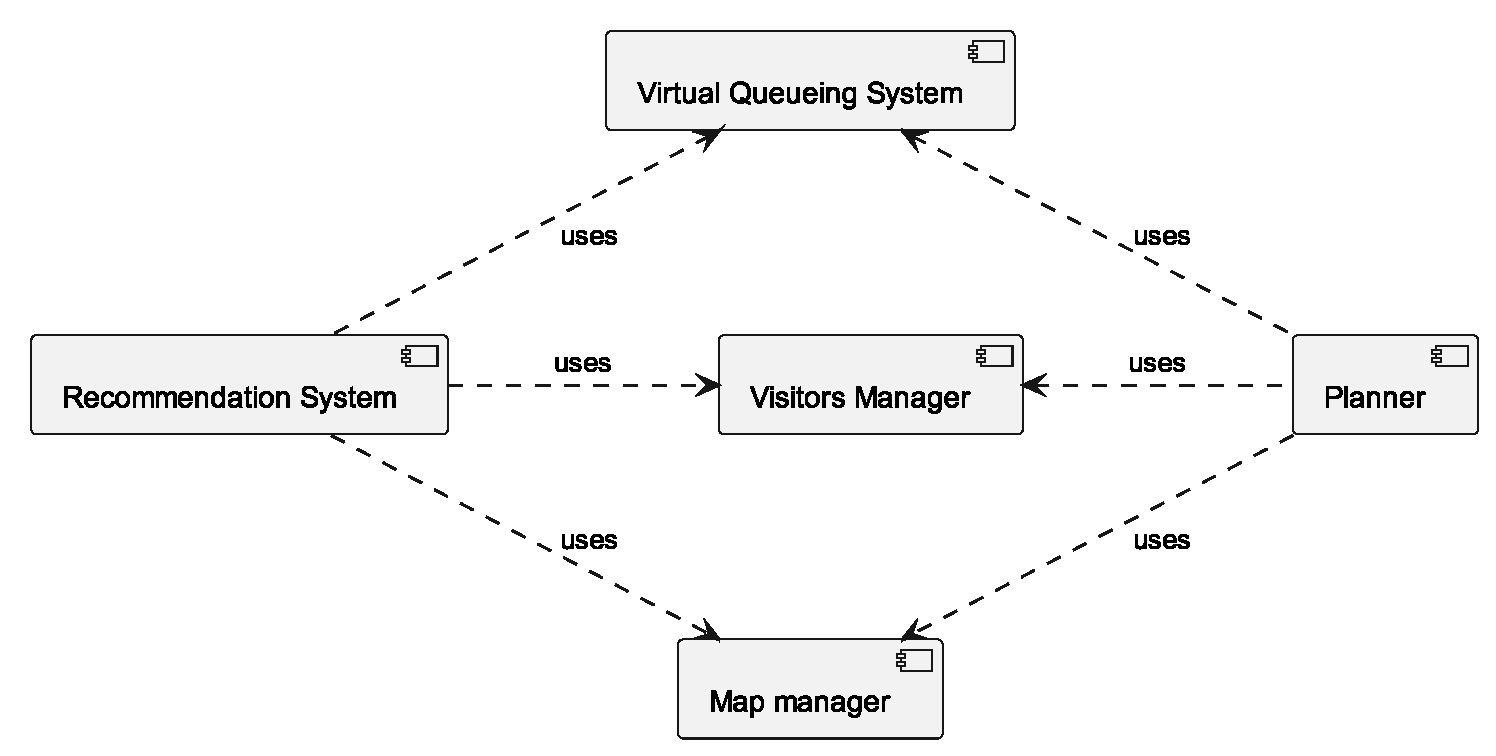
\includegraphics[width=0.9\textwidth]{img/architecture-overview.eps}
	\caption{Overview architecture of Mirabilandia as a micro-city.
		The component diagram shows the rough architecture in the context of Mirabilandia, showing the main dependencies between them.
	}
	\label{fig:architecture-overview}
\end{figure}

Following the analysis of the ``as-is'' system and the goals set % TODO write the goals?
to adapt the smart micro-city concept to Mirabilandia, the figure~\ref{fig:architecture-overview} shows the component diagram that models the entities involved and the main relationships between them.

The main components of the system are the following:

\begin{itemize}
	\item \textit{Map Manager}: is responsible for tracking the guest within the park and providing information about the current position
	\item \textit{Virtual Queueing System}: is responsible for managing the virtual queue for each attraction
	\item \textit{Recommendation System}: is responsible for providing recommendations to the visitors based on different factors that will be further discussed in the next sections.
	\item \textit{Planner}: is responsible for planning the itinerary of the guests based on their preferences and crowding of rides
\end{itemize}

From the diagram emerge that \textit{Map Manager} and \textit{Virtual Queueing System} are the main components of the system since they are the ones
that provide information to the other components. The \textit{Map Manager} provides information about the current position of the guests
to the \textit{Recommendation System} which uses this information to provide recommendations to the guests. Moreover, gives information also to the
\textit{Planner} to avoid crowd situations and maintain a uniform distribution of guests in the park. The \textit{Virtual Queueing System} is used by
the \textit{Planner} to plan the itinerary of the guests and adapt it to reduce the waiting time and improve the quality of the visit within the park
and by the \textit{Recommendation System} to fetch information about the current waiting time of the attractions and opportunistically advise the attraction.
% TODO fix the section considering the Visitor Manager

\section{Map Manager}

The location of guests within the amusement park is critical for several reasons: guest location information is used to make recommendations and to determine the best plan for each guest. So, good tracking is crucial for the good working of the overall system.

\begin{figure}[H]
	\centering
	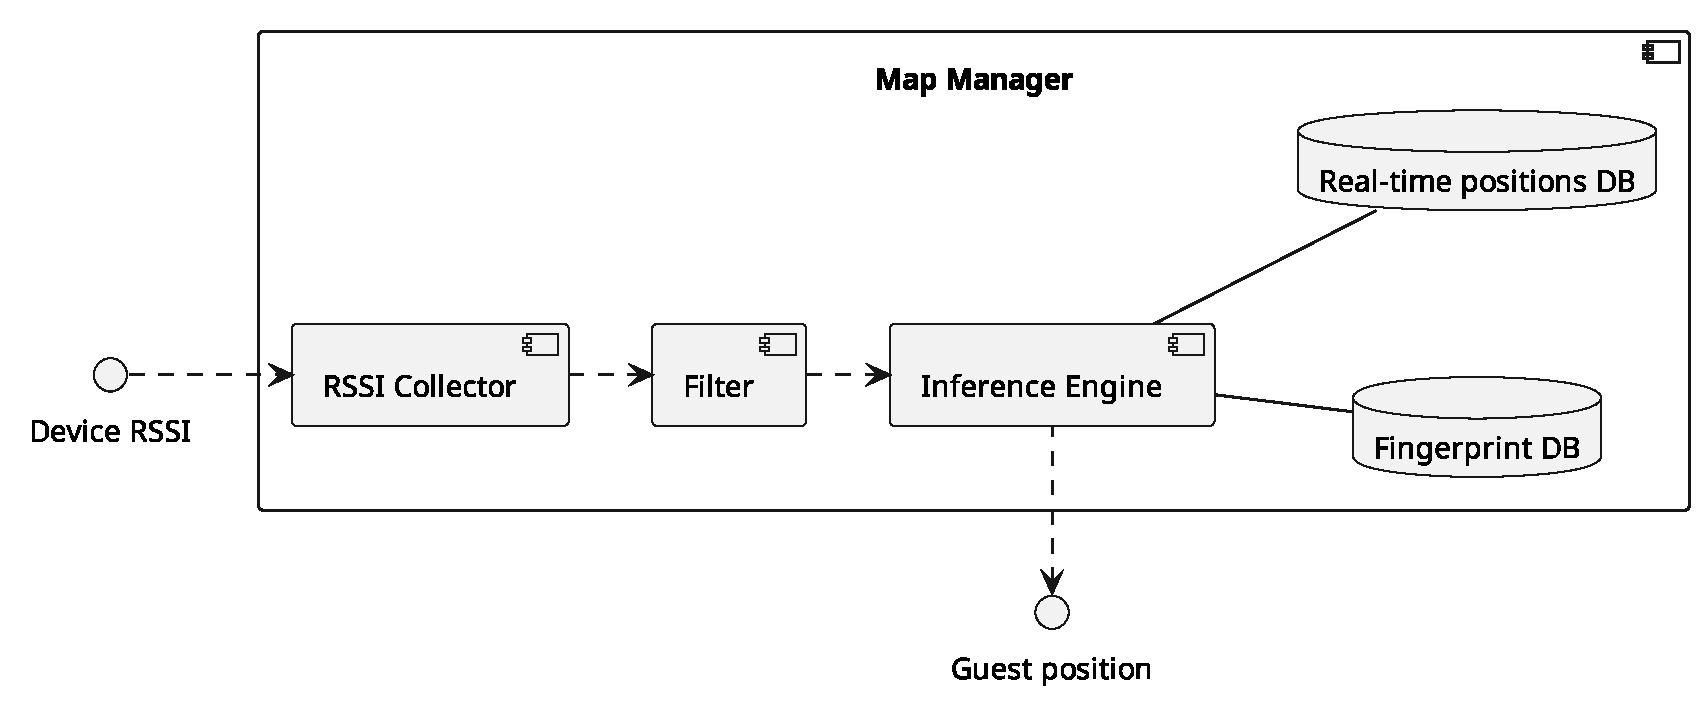
\includegraphics[width=\textwidth]{img/map-manager.eps}
	\caption{Component diagram showing the internal architecture of the \textit{Map Manager} component.
	}
	\label{fig:map-manager}
\end{figure}

\subsection{Technologies for visitors localization}\label{sec:technologies}
Visitors localization could be useful for both proximity marketing and calculating the number of people in a queue.
Indoor localization could be helpful in our context as there are restaurants, shops and some attractions
(e.g.\ Reset\footnote{\url{https://www.mirabilandia.it/en/attivita/attrazioni/reset}}) not easily reached by the outdoor localization technologies.
Moreover, the accuracy of outdoor localization technologies (e.g.\ GPS) may not be enough accurate for instance for the prize games area\footnote{\url{https://www.mirabilandia.it/en/attivita/attrazioni/altri-giochi-e-giochi-a-premio}}
where the stands are located next to each other.

Some technologies identified for these purposes will be described in the following sections.

\subsubsection{Wi-Fi as outdoor localization system}\label{subsec:wi-fi-as-outdoor-localization-system}

Wi-Fi is a family of wireless network protocols, which are commonly used for local area networking of devices and Internet access, allowing nearby digital device to exchange data by radio waves.

To date, Wi-Fi is a technology that has been pervasively adopted and made accessible to anyone because of cost, ease of installation and configuration.

Unlike other technologies such as the global positioning system (GPS), Wi-Fi was not designed to perform device and/or person location.
However, by exploiting ad-hoc techniques it is possible to leverage this tool to perform device localization.
Finally, GPS does not always perform well in any context: in closed environments or where the GPS signal cannot reach, localization using
this technology is approximate or even impractical.
Another problem with GPS is its high power consumption, which is a serious challenge to battery-based mobile devices.
To tackle the problems with GPS, many researchers have proposed a series of alternative localization schemes, including cellular-based systems~\cite{ibrahim2010cellsense},
infrared-based systems, ultrasonic-based systems, and radio frequency (RF)-based systems~\cite{bahl2000radar, youssef2002probabilistic}.

Many researchers have proposed a variety of different schemes for outdoor localization based on mobile
devices.
These schemes can be divided into two groups: range-based and range-free methods.

\begin{itemize}
	\item \textbf{Range-based}: range-based methods are mainly based on relative distance, which can be obtained through measuring methods like time-of-arrival (ToA),
	      time difference of arrival (TDoA), or propagation model generated from RSSI value.
	\item \textbf{Range-free}: one of the most widely used range-free method is fingerprint localization method.
	      This method can be categorized into three types:
	      visual fingerprint-based localization, motion fingerprint-based systems, and signal fingerprint-based methods.
	      In our context the latter is the most promising.
\end{itemize}

\subsubsection{Signal fingerprint-based localization}
Signal fingerprint-based localization is widely used in places where a large number of Wi-Fi infrastructures are deployed.
This methods commonly consist of offline training phase and online fingerprint matching phase.
The goal of the first phase is to form a fingerprint database which stores the correlation between \textit{Received Signal Strength} (RSS) from
various \textit{Access Points}(APs) and fixed locations.
The device's location is determined at the matching stage.
In this process we use matching algorithm to search the fingerprint
in the database which has the minimum difference with the device that needs to be located.
The associated label is our estimated location.

\subsubsection{Signal fingerprint-based localization improvement with NFC technology}
In terms of effect, signal fingerprint-based localization has the ability to get fine-grained results.
However, as any radio environment is dynamic: unpredictable movements of the people or large unforeseen gatherings,
alterations in the radio network itself, and environmental effects such as change in humidity levels etc.~\cite{chaudhry2013indoor}
Therefore, the RF values measured for location estimation at any given point in time may significantly deviate from
those stored in the database created at the training phase~\cite{chaudhry2013indoor}.
As a result, the location estimation based on a static database may be inaccurate.
Also, the training phase needs a human operator (or a human-assisted machine) to thoroughly collect the RF context and
the location at which the context was collected from.
To tackle these problems, as suggested in~\cite{chaudhry2013indoor}, it could be useful a system which considers the NFC technology:
reference points of precisely known locations are spread in the environment, marked by NFC tags, to build the database of fingerprints around.
This could improve the training phase and allows easy adaptation to environmental changes.

\subsubsection{Bluetooth as outdoor localization system}
Bluetooth is a data transmission standard for personal wireless networks. It provides a standard way to exchange information between
devices through a short-range frequency capable of detecting devices covered by the radio signal within about ten meters by putting them
in communication with each other.

Despite being a technology conceived more than 20 years ago, it boasts massive adoption in many contexts such as medical, industrial, and in
recent years in the Internet of Things (IoT). This standard was designed with the goal of achieving low power consumption, short range
and a low cost of production. Over the years, there have been several updates to the protocol, aimed at improving on the one hand the efficiency of
communication by enabling higher transmission frequencies and on the other hand improving the energy efficiency of devices.

Bluetooth was not designed to perform localization functionality. However, it is possible to exploit certain
features of the protocol to make a more or less precise estimate of a device's location. In particular, the technique most
used to achieve this is based on the signal strength identified by the RSSI (Receives Signal Strength Indicator).
Other techniques, such as fingerprint-based localization can be employed to estimate position.

With the RSSI-based technique, the RSSIs of all reachable Bluetooth devices are initially acquired, and through techniques of trilateration, the
location of the device is estimated.\\
Fingerprint-based techniques estimate the location by operating in two stages: the first is the training phase that deals with building fingerprints,
which is a record that associates a location with the RSSIs of beacons reachable from that
point. The second phase involves identifying the fingerprint that least deviates from the position where the device is at a given time, and the
position associated to that fingerprint determines the estimated position. Several projects and applications rely on these two techniques to estimate
the position of a device~\cite{mcconville2021vesta, samuel2021smart}.

The proliferation of location services for various IoT applications needs to detect device locations with very high accuracies, on the order of
centimeters. With the introduction of the Bluetooth 5.1 standard, a new feature called \textit{Direction Finding} that enables pinpoint localization
of Bluetooth devices.
This new localization feature provides two different options for positioning a Bluetooth device, namely Angle of Arrival (AoA) and Angle of Departure
(AoD) compared to the previous version that relies only on the received signal strength indication to localize a Bluetooth device.
To be more precise, the former technique allows a receiver equipped with a multi-antenna array to identify the angular position of a transmitter
based on the phase delay of the signal received from the transmitter; the latter allows the transmitting device with multiple antennas to transmit a
radio signal that permits the receiver to determine the directional angle to the transmitter

\subsection{Suitable localization techniques for Mirabilandia}
% Il resto della sezione la sposterei in una sezione successiva in cui identifichiamo la tecnologia migliore per il tracciamento delle persone. 
% A new approach in signal fingerprint-based localization is proposed in~\cite{du2018hybrid}. In the article they propose the following technique to stimate the position
% of a device: we use $f = {r_1, r_2, \ldots, r_n}$ to indicate a \textit{fingerprint} where $r_i$ represents the RSS value of captured AP and $n$ the number of APs in the fingerprint.
% We calculate the dissimilarity between two fingerprints based on RSS difference. Denote with $\sigma_i = | r_i - r^{'}_{i}|$ the difference of fingerprints $f^{'}$ and $f$ at each $A_i$ where
% $A_i \in A$ where $A$ is the fingerprint's APs set. Due to the fact that two fingerprints may contain different set of APs, so it may appear that AP $A_i$ appears in $f$ but
% does not appear in $f^{'}$. For this situation, we assume the signal strength is weak and let the missing value equal to $-100$. The dissimilarity between $f$ and $f^{'}$ can be shown as:

% \begin{equation}
%     \eta(f, f^{'}) = \sqrt{\sum_{i=0}^{p} \sigma_i^{2}}
% \end{equation}

% where $p = | A \cup A^{'} |$

% We found the sample with minimum dissimilarity through compare all samples stored in the fingerprint database $F$ with the query fingerprint $f$.

% \begin{equation}
%     f^{*} = \arg \max_{f_i \in F} \ \eta(f, f_i)
% \end{equation}

% $L(f^{*})$ is the corresponding location of $f^{*}$ which represent the estimated place.

%TODO \subsection{Virtual Queueing - technologies for waiting time etimation}
%TODO \subsection{Queue length estimation: NFC(people scanning a tag letting know they are there) vs Bluetooth(automatically doing that)} ??

\section{Virtual Queuing System}
\begin{figure}[H]
	\centering
	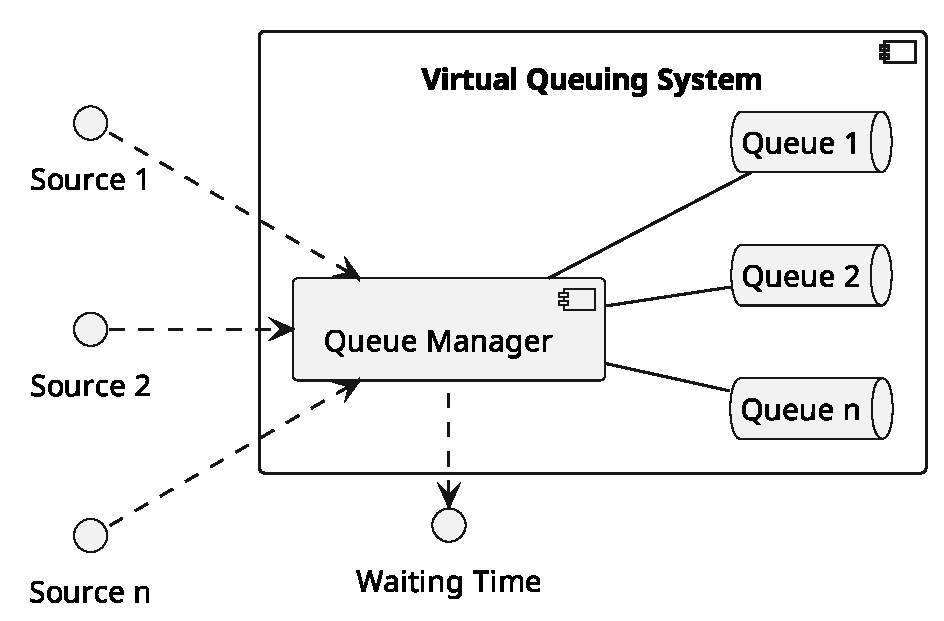
\includegraphics[width=0.6\textwidth]{img/virtual-queuing.eps}
	\caption{Component diagram showing the internal architecture of the \textit{Virtual Queueing} component.
	}
	\label{fig:virtual-queueing-arch}
\end{figure}

\section{Recommendation System}
The Recommendation System is a crucial component to ensure the improvement of the visitors' experience.
In fact, it is responsible for collecting data and providing tailored recommendations to the visitors
and uses a Reward System to provide rewards based on the suggested actions.
The Recommendation System is composed of:
Attractions (i.e. roller coasters, restaurants, shops, etc.) and Shows
\begin{itemize}
	\item a \textit{Attractions Recommender}
	\item a \textit{Shows Recommender} which takes visitor's information from the Visitor Manager to get their pre-compiled preferences about the shows they are interest in, and from the Map Manager, to get the visitor's location and send a notification based on their proximity to a point of interest.
\end{itemize}


Due to its "situatedness" nature, is triggered by the presence of a suitable visitor in a place of interest.

The Reward System collects all the rewards to be given to the visitors and the Recommender (which knows the visitor's preferences)
decide which one to send.

\begin{figure}[H]
	\centering
	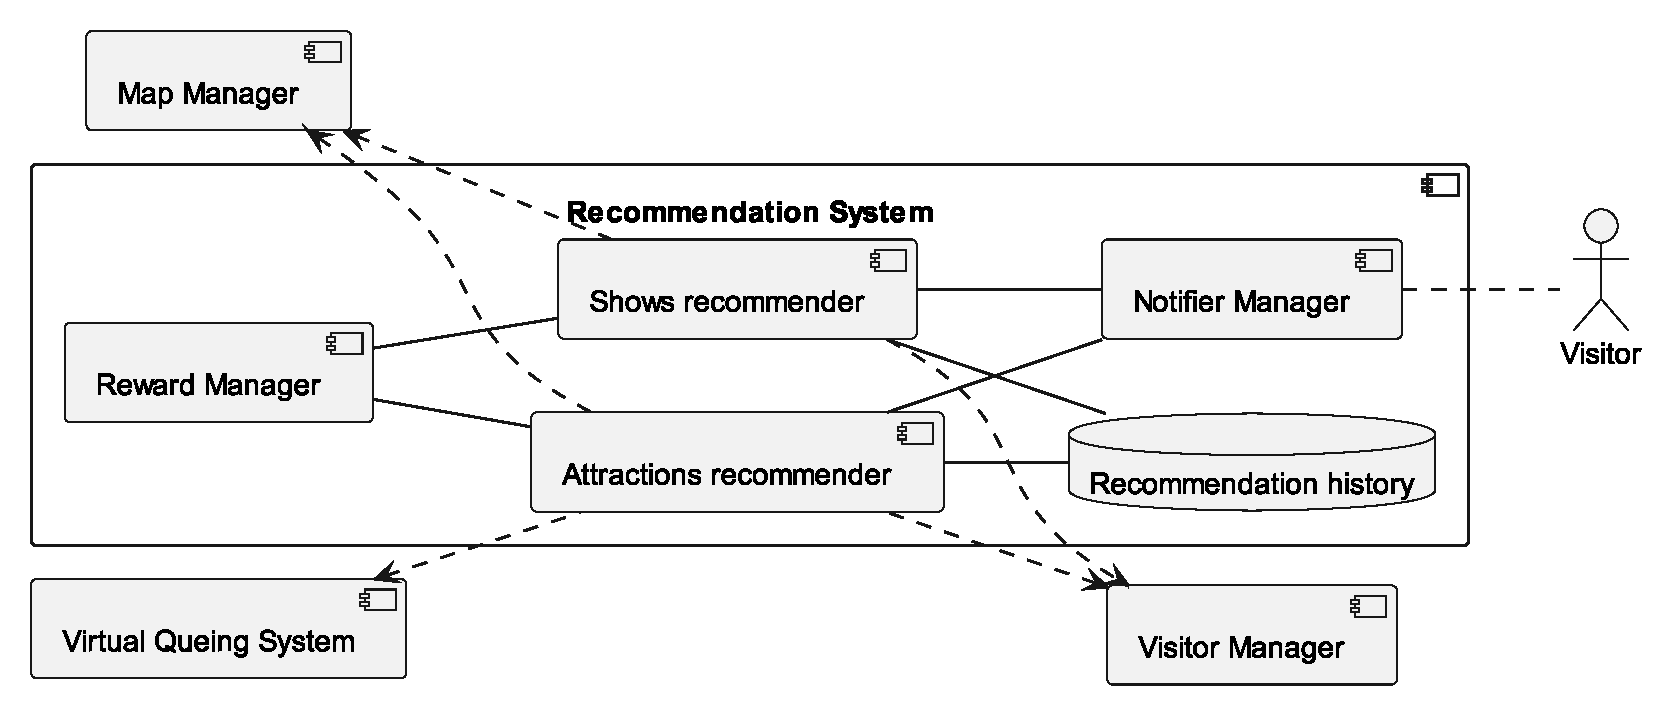
\includegraphics[width=0.9\textwidth]{img/recommender.eps}
	\caption{Component diagram showing the internal architecture of the \textit{Recommender System} component.
	}
	\label{fig:recommender-arch}
\end{figure}

\subsection{Proximity Marketing with WiFi}\label{subsec:technologies-for-proximity-marketing}
Proximity-driven marketing systems have mostly been developed with the use of Bluetooth beacons~\cite{mndebele2017iot}.
However, it is possible to enable IoT-based proximity communication running as a service using network information, exploiting WiFi.
This offers better value than Bluetooth in terms of efficiency and cost-effectiveness, as it can be used to implement IoT-based proximity solutions that run on existing infrastructure.
The detection of Wi-Fi networks already provides some data about location, namely information about proximity so
proximity-based rules replace location information, where Wi-Fi hot spots work as presence sensors~\cite{dmitry2013network}.

This paper~\cite{mndebele2017iot} for instance, presents a proximity marketing as a service (PMaas) system that targets people in a specific location and delivers messages to their mobile devices via wireless connectivity technology as long as they remain in the specified location and only while they are connected to a particular network segment or specific access point.
To do so, the system uses network information, i.e. the network name, and GPS parameters derived from the position of the mobile device.
The marketing messages are sent by a cloud-based platform to the eligible devices and a mobile app listens for messages
applicable to the subscriber, while the subscriber is in the relevant proximity.


\section{Planner}

\begin{figure}[H]
	\centering
	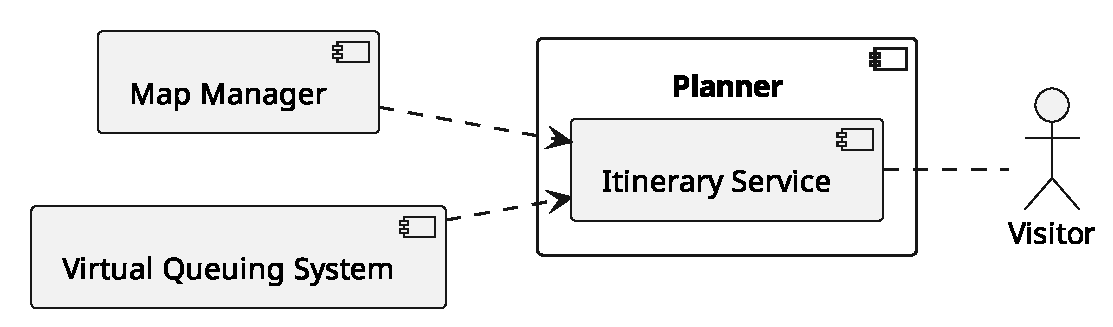
\includegraphics[width=0.7\textwidth]{img/planner.eps}
	\caption{Component diagram showing the internal architecture of the \textit{Planner} component.
	}
	\label{fig:planner-arch}
\end{figure}

\subsection{Sub-GHz Wireless Sensor Network for crowd density estimation}\label{subsec:sub-ghz-wireless-sensor-network-for-crowd-density-estimation}
In our context, crowd density estimation could be advantageous to redirect visitors toward less crowded places within the park.
The classic approach to obtaining this information is to make use of an optical camera-based system but the accuracy of these systems can be
rather dependent on the lighting conditions and they tend to require the availability of a large amount of computing power.
Furthermore, the use of optical cameras raises the spectre of privacy-related issues.
A WSN-based system could potentially be used to simply avoid these issues~\cite{denis2018large}.
In fact, the use of sub-GHz frequencies could be the best decision, due to their increased range and penetration capabilities through objects, walls and human individuals~\cite{denis2018large}.
Moreover, this kind of transceivers, compared to the regular WiFi, have a significant lower power-consumption~\cite{fudickar2014comparing}.

As presented in~\cite{denis2018large}, they managed to show the feasibility of using a sub-GHz wireless network to estimate the
density of large-scale crowds calculating the mean RSS-differences within a WSN between an empty and an active environment and used them
as input to a probabilistic neural network.
Whereas in~\cite{fudickar2014comparing}, showed that Sub GHz transceivers achieve significant lower RSS errors and are less influenced by obstacles attenuations.
Their localisation achieved ca. 1 m more accurate median error distances than the corresponding versions that utilise WiFi transceivers.
In addition, the battery runtimes are extended by 48\% when using Sub GHz transceivers instead of WiFi transceivers.


\section{Visitors Manager}

\begin{figure}[H]
	\centering
	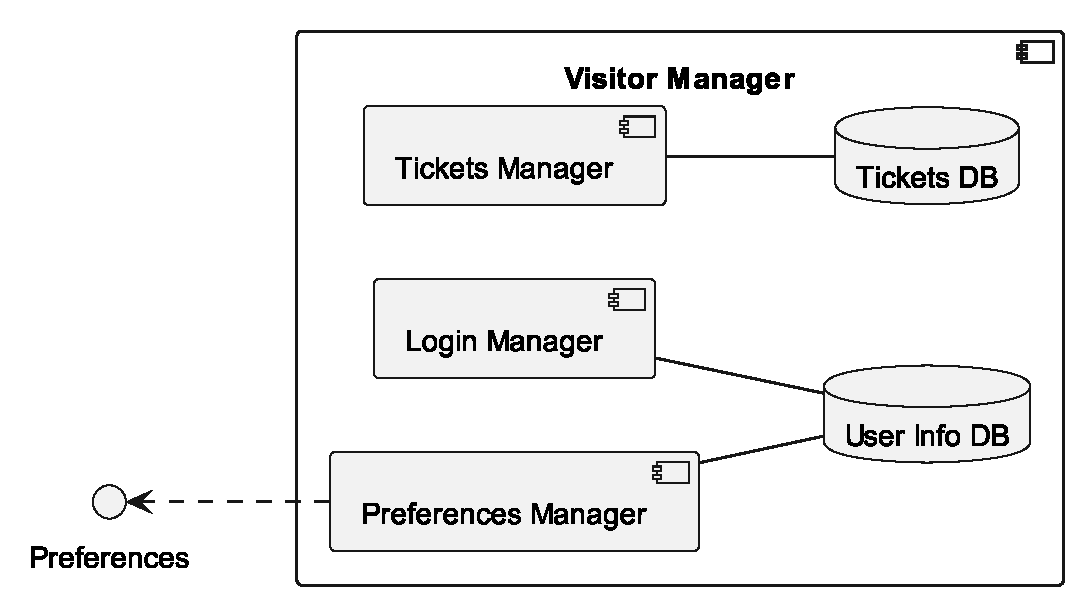
\includegraphics[width=0.7\textwidth]{img/visitor-manager.eps}
	\caption{Component diagram showing the internal architecture of the \textit{Visitor Manager} component.
	}
	\label{fig:visitor-manager-arch}
\end{figure}